\section{Introducing differentiable binary arithmetic operations}
\label{sec:Nalu}
We define our problem as learning a set of static arithmetic operations between selected elements of a vector. E.g. for a vector $\mathbf{x}$ learn the function ${(x_5 + x_1) \cdot x_7}$. The approach taking in this paper, is to develop layers around specific operations, and then let each layer decide which inputs to include using backpropagation.

We develop these layers by taking inspiration from an theoretical analysis of Neural Arithmetic Logic Unit (NALU) by \citet{trask-nalu}.

\subsection{Introducing NALU}
The Neural Arithmetic Logic Unit (NALU) consists of two sub-units; the $\text{NAC}_{+}$ and $\text{NAC}_{\bullet}$. These represent either the $\{+, -\}$ or the $\{\times, \div \}$ operations. The NALU then assumes that either $\text{NAC}_{+}$ or $\text{NAC}_{\bullet}$ will be selected exclusively, using a sigmoid gating-mechanism.

The $\text{NAC}_{+}$ and $\text{NAC}_{\bullet}$ are defined accordingly,
\begin{align}
W_{h_\ell, h_{\ell-1}} &= \tanh(\hat{W}_{h_\ell, h_{\ell-1}}) \sigma(\hat{M}_{h_\ell, h_{\ell-1}}) \label{eq:weight}\\
\textrm{NAC}_+:\ z_{h_\ell} &= \sum_{h_{\ell-1}=1}^{H_{\ell-1}} W_{h_{\ell}, h_{\ell-1}} z_{h_{\ell-1}} \label{eq:naca}\\
\textrm{NAC}_\bullet:\ z_{h_\ell} &= \exp\left(\sum_{h_{\ell-1}=1}^{H_{\ell-1}} W_{h_{\ell}, h_{\ell-1}} \label{eq:nacm}\log(|z_{h_{\ell-1}}| + \epsilon) \right)
\end{align}
where $\hat{\mathbf{W}}, \hat{\mathbf{M}} \in \mathbb{R}^{H_{\ell} \times H_{\ell-1}}$ are weight matrices and $z_{h_{\ell-1}}$ is the input. The matrices are combined using a tanh-sigmoid transformation to bias the parameters towards a $\{-1,0,1\}$ solution. Having $\{-1,0,1\}$ allows $\text{NAC}_{+}$ to be perform exact $\{+, -\}$ operations between elements of a vector.
The $\text{NAC}_{\bullet}$ uses an exponential-log transformation to create the $\{\times, \div \}$ operations (within $\epsilon$ precision).

The NALU combines these units with a gating mechanism $\mathbf{z} = \mathbf{g} \odot \text{NAC}_{+} + (1 - \mathbf{g}) \odot \text{NAC}_{\bullet}$ given $\mathbf{g} = \sigma(\mathbf{G} \mathbf{x})$. Thus allowing NALU to decide between all of $\{+, -, \times, \div\}$ using backpropagation.

\subsection{Weight matrix construction  and the Neural Addition Unit}\label{sssec:weight}

\citet{glorot-initialization} show that $E[z_{h_\ell}] = 0$ at initialization is a desired property, as it prevents explosion of both the output and the gradients. To satisfy this property with $W_{h_{\ell-1},h_\ell} = \tanh(\hat{W}_{h_{\ell-1},h_\ell}) \sigma(\hat{M}_{h_{\ell-1},h_\ell})$, an initialization must satisfy $E[\tanh(\hat{W}_{h_{\ell-1},h_\ell})] = 0$. In the context of NALU, this initialization is also unbiased as it samples evenly between $+$ and $-$, or $\times$ and $\div$. Unfortunately, this initialization also causes the expectation of the gradient to become zero, as shown in \eqref{eq:nac-weight-gradient}.

\begin{equation}
E\left[\frac{\partial \mathcal{L}}{\partial \hat{M}_{h_{\ell-1},h_\ell}}\right] = E\left[\frac{\partial \mathcal{L}}{\partial W_{h_{\ell-1},h_\ell}}\right] E\left[\tanh(\hat{W}_{h_{\ell-1},h_\ell})\right] E\left[\sigma'(\hat{M}_{h_{\ell-1},h_\ell})\right] = 0
\label{eq:nac-weight-gradient}
\end{equation}

Besides the issue of initialization, our empirical analysis (table \ref{tab:function-task-static-defaults}) shows that this weight construction \eqref{eq:weight} does not create the desired bias for $\{-1, 0, 1\}$ for the addition and subtraction problem.

To solve these issues, we add a sparsifying regularizer to the loss function ($\mathcal{L} = \hat{\mathcal{L}} + \lambda_{\mathrm{sparse}} \mathcal{R}_{\ell,\mathrm{sparse}}$) and use simple linear weight construction, where $W_{h_{\ell-1},h_\ell}$ is clamped to $[-1, 1]$ in each iteration.

\begin{align}
W_{h_{\ell-1},h_\ell} &= \min(\max(W_{h_{\ell-1},h_\ell}, -1), 1), \\
\mathcal{R}_{\ell,\mathrm{sparse}} &= \frac{1}{H_\ell \cdot H_{\ell-1}} \sum_{h_\ell=1}^{H_\ell} \sum_{h_{\ell-1}=1}^{H_{\ell-1}} \min\left(|W_{h_{\ell-1},h_\ell}|, 1 - \left|W_{h_{\ell-1},h_\ell}\right|\right) \\
\textrm{NAU}:\ z_{h_\ell} &= \sum_{h_{\ell-1}=1}^{H_{\ell-1}} W_{h_{\ell}, h_{\ell-1}} z_{h_{\ell-1}}
\end{align}

\subsection{Challenges of division} \label{sssec:nac-mul}

The $\text{NAC}_{\bullet}$, as formulated in equation \ref{eq:nacm}, has the ability to perform exact multiplication and division, or more precisely multiplication of the inverse of elements from a vector, when a weight in $W_{h_{\ell-1},h_\ell}$ is $-1$.

However, this flexibility creates critical optimization challenges. Expanding the exp-log-transformation, $\text{NAC}_{\bullet}$ can be express as
\begin{equation}
\textrm{NAC}_\bullet:\ z_{h_\ell} = \prod_{h_{\ell-1}=1}^{H_{\ell-1}} (|z_{h_{\ell-1}}| + \epsilon)^{W_{h_{\ell}, h_{\ell-1}}}\ .
\label{eq:division:nac-mul-rewrite}
\end{equation}

In equation \eqref{eq:division:nac-mul-rewrite}, if $|z_{h_{\ell-1}}|$ is near zero ($E[z_{h_{\ell-1}}] = 0$ is a desired property when initializing \cite{glorot-initialization}), $W_{h_{\ell-1},h_\ell}$ is negative, and $\epsilon$ is small, then the output will explode. This issue is present even for a reasonably large $\epsilon$ value (such as $\epsilon = 0.1$), and just a slightly negative $W_{h_{\ell-1},h_\ell}$, as visualized in figure \ref{fig:nac-mul-eps-issue}. Also note that the curvature can cause convergence to an unstable area.

This singularity issues in the optimization space also makes multiplication challenging, which further suggests that supporting division is infeasible. These observations are also found empirically in (see \citet{trask-nalu}, table 1 and Appendix \ref{sec:appendix:comparison-all-models}).

%However, backpropagation through the $\text{NAC}_{\bullet}$ unit (equation \ref{eq:dz}, derivation in Appendix \ref{sec:appendix:gradient-derivatives:gradient-nac-mul}) reveals that if $|z_{h_{\ell-1}}|$ is near zero, $W_{h_{\ell-1},h_\ell}$ is negative and $\epsilon$ is small, the gradient term will explode and oscillate between large positive and large negative values, which can be problematic in optimization \cite{adam-optimization}, as visualized in figure \ref{fig:nac-mul-eps-issue}.
%\begin{align}
%\frac{\partial \mathcal{L}}{\partial W_{h_{\ell}, h_{\ell - 1}}} &= \frac{\partial \mathcal{L}}{\partial z_{h_\ell}} \frac{\partial z_{h_\ell}}{\partial W_{h_{\ell}, h_{\ell - 1}}} = \frac{\partial \mathcal{L}}{\partial z_{h_\ell}} z_{h_\ell} \log(|z_{h_{\ell-1}}| + \epsilon) \label{eq:dw}\\
%\frac{\partial \mathcal{L}}{\partial z_{h_{\ell-1}}} &= \sum_{h_\ell = 1}^{H_\ell} \frac{\partial \mathcal{L}}{\partial z_{h_\ell}} \frac{\partial z_{h_\ell}}{\partial z_{h_{\ell-1}}} = \sum_{h_\ell = 1}^{H_\ell} \frac{\partial \mathcal{L}}{\partial z_{h_\ell}} z_{h_\ell} W_{h_\ell, h_{\ell-1}} \frac{\mathrm{sign}(z_{h_{\ell-1}})}{|z_{h_{\ell-1}}| + \epsilon}\label{eq:dz}
%\end{align}

%This is not an issue for positive values of $W_{h_{\ell-1},h_\ell}$ (multiplication), as $z_{h_{\ell}}$ and $z_{h_{\ell-1}}$ will be correlated causing the terms $z_{h_\ell}$ and $\frac{\mathrm{sign}(z_{h_{\ell-1}})}{|z_{h_{\ell-1}}| + \epsilon}$ to partially cancel out.

% This gradient can be particular problematic when considering that $E[z_{h_{\ell-1}}] = 0$ is a desired property when initializing \cite{glorot-initialization}.
% A desired multiplication unit should not explode for $z_{h_{\ell-1}}$ near zero, which is why supporting division is likely infeasible.

\begin{figure}[h]
\centering
\begin{subfigure}{.33\textwidth}
  \centering
  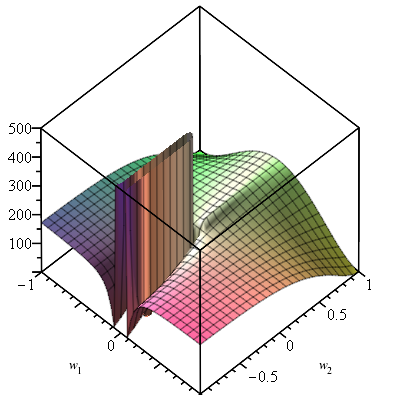
\includegraphics[width=\linewidth,trim={0 0 0 4.35cm},clip]{graphics/nac-mul-eps-1em7.png}
  \caption{$\mathrm{NAC}_{\bullet}$ with $\epsilon = 10^{-7}$}
\end{subfigure}%
\begin{subfigure}{.33\textwidth}
  \centering
  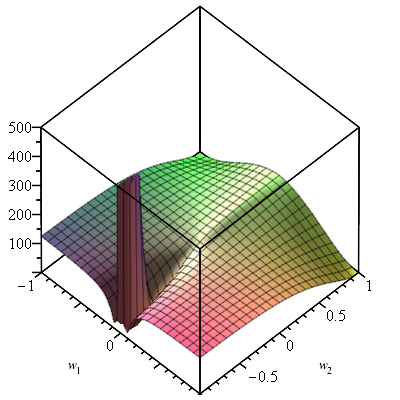
\includegraphics[width=\linewidth,trim={0 0 0 4.35cm},clip]{graphics/nac-mul-eps-1em1.png}
  \caption{$\mathrm{NAC}_{\bullet}$ with $\epsilon = 0.1$}
\end{subfigure}
\begin{subfigure}{.33\textwidth}
  \centering
  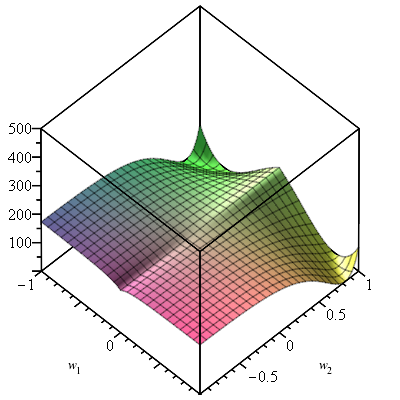
\includegraphics[width=\linewidth,trim={0 0 0 4.35cm},clip]{graphics/nac-mul-eps-1.png}
  \caption{$\epsilon = 1$}
\end{subfigure}
%\begin{subfigure}{.33\textwidth}
%  \centering
%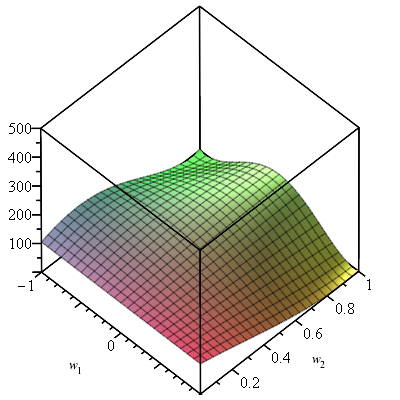
\includegraphics[width=\linewidth]{graphics/nac-mul-nmu.png}
%  \caption{Our NMU solution}
%\end{subfigure}

\caption{RMS loss curvature for a $\mathrm{NAC}_{+}$ layer followed by a $\mathrm{NAC}_{\bullet}$. The weight matrices are constrained to $\mathbf{W}_1 = \left[\protect\begin{smallmatrix}
w_1 & w_1 & 0 & 0 \\
w_1 & w_1 & w_1 & w_1
\protect\end{smallmatrix}\right]$, $\mathbf{W}_2 = \left[\protect\begin{smallmatrix}
w_2 & w_2
\protect\end{smallmatrix}\right]$. The problem is $(x_1 + x_2) \cdot (x_1 + x_2 + x_3 + x_4)$ for $x = \left(1, 1.2, 1.8, 2\right)$. The solution is $w_1 = w_2 = 1$, with many unstable solutions.}
\label{fig:nac-mul-eps-issue}
\end{figure}

\subsection{Initialization of \texorpdfstring{$\mathrm{NAC}_{\bullet}$}{NAC-mul}}
Initialization is important to consider for fast and consistent convergence, one desired property is that weights can be initialized such that $E[z_{h_\ell}] = 0$ \cite{glorot-initialization}. Using second order Taylor approximation and assuming all $z_{h_{\ell-1}}$ are uncorrelated; the expectation of $\mathrm{NAC}_{\bullet}$ can be estimated as
\begin{equation}
E[z_{h_\ell}] \approx \left(1 + \frac{1}{2} Var[W_{h_\ell, h_{\ell-1}}] \log(|E[z_{h_{\ell-1}}]| + \epsilon)^2\right)^{H_{\ell-1}} \Rightarrow E[z_{h_\ell}] > 1.
\label{eq:nac-mul:expectation}
\end{equation}
As shown in equation \ref{eq:nac-mul:expectation}, satisfying $E[z_{h_\ell}] = 0$ for $\mathrm{NAC}_{\bullet}$ is likely impossible. The variance can also not be input-independent initialized and is expected to explode (proofs in Appendix \ref{sec:appendix:moments:nac-mul}).

\subsection{Neural multiplication unit}
To solve the the gradient and initialization challenges for $\mathrm{NAC}_{\bullet}$ we propose a new neural multiplication unit (NMU):

\begin{align}
W_{h_{\ell-1},h_\ell} &= \min(\max(W_{h_{\ell-1},h_\ell}, 0), 1), \\
\mathcal{R}_{\ell,\mathrm{sparse}} &= \frac{1}{H_\ell \cdot H_{\ell-1}} \sum_{h_\ell=1}^{H_\ell} \sum_{h_{\ell-1}=1}^{H_{\ell-1}} \min\left(W_{h_{\ell-1},h_\ell}, 1 - W_{h_{\ell-1},h_\ell}\right) \\
\textrm{NMU}:\ z_{h_\ell} &= \prod_{h_{\ell-1}=1}^{H_{\ell-1}} \left(W_{h_{\ell-1},h_\ell} z_{h_{\ell-1}} + 1 - W_{h_{\ell-1},h_\ell} \right) \label{eq:nmu-defintion}
\end{align}
The NMU is regularized similar to the NAU and has a multiplicative identity when $W_{h_{\ell-1},h_\ell}=0$.
The NMU unit does not support division by design.
%Previous experiments using the NALU for division does not work well on division hence very little is lost with this modification \cite{trask-nalu}.
As opposed to the $\mathrm{NAC}_{\bullet}$, the NMU can represent input of both negative and positive values and is not $\epsilon$ bounded, which allows the NMU to extrapolate to $z_{h_{\ell-1}}$ that are negative or smaller than $\epsilon$. Its gradients are derived in Appendix \ref{sec:appendix:gradient-derivatives:gradient-nmu}.

\subsection{Moments and initialization}
The NAU is a linear layer and can be initialized using \citet{glorot-initialization}. The $\mathrm{NAC}_{+}$ unit can also achieve an ideal initialization, although it is less trivial (details in Appendix \ref{sec:appendix:moments:weight-matrix-construction}).

The NMU is initialized with $E[W_{h_{\ell}, h_{\ell - 1}}] = \nicefrac{1}{2}$. Assuming all $z_{h_{\ell-1}}$ are uncorrelated, and $E[z_{h_{\ell-1}}] = 0$, which is the case for most neural units \cite{glorot-initialization}, the expectation can be approximated to
\begin{equation}
E[z_{h_\ell}] \approx \left(\frac{1}{2}\right)^{H_{\ell-1}},
\end{equation}
which approaches zero for $H_{\ell-1} \rightarrow \infty$ (see Appendix \ref{sec:appendix:moments:nmu}). The NMU can, assuming $Var[z_{h_{\ell-1}}] = 1$ and $H_{\ell-1}$ is large, be optimally initialized with $Var[W_{h_{\ell-1},h_\ell}] = \frac{1}{4}$ (proof in Appendix \ref{sec:appendix:moments:nmu:initialization}).

\subsection{Regularizer scaling}
We use the regularizer scaling as defined in \eqref{eq:regualizer-scaling}. We motivate this by observing optimization consists of two parts. A warmup period, where $W_{h_{\ell-1},h_\ell}$ should get close to the solution, unhindered by the sparsity regularizer, and then a period where the solution is made sparse.
\begin{equation}
\lambda_{\mathrm{sparse}} = \hat{\lambda}_{\mathrm{sparse}} \max\left(\min\left(\frac{t - \lambda_{\mathrm{start}}}{\lambda_{\mathrm{end}} - \lambda_{\mathrm{start}}}, 1\right), 0\right)
\label{eq:regualizer-scaling}
\end{equation}

\subsection{NALU: Challenges of gating between \texorpdfstring{$\text{NAC}_{+}$}{NAC-add} and \texorpdfstring{$\text{NAC}_{\bullet}$}{NAC-mul}}
\label{sec:methods:gatting-issue}
The purpose of the gating-mechanism is to select either $\text{NAC}_{+}$ or $\text{NAC}_{\bullet}$ exclusively.
This assumes that the correct sub-unit is selected by the NALU, since selecting the wrong sub-unit leaves no gradient signal for the correct sub-unit.

Empirically we find this assumption to be problematic.
We observe that both sub-units converges in the beginning of training whereafter the gating-mechanism, seamlessly randomly, converges towards either the $\text{NAC}_{+}$ or $\text{NAC}_{\bullet}$ (in-depth empirical analysis in appendix \ref{sec:appendix:nalu-gate-experiment}, with results for both a shared and non-shared weight matrix between $\text{NAC}_{+}$ and $\text{NAC}_{\bullet}$).

As the problem size grows, randomly choosing the correct gating value becomes an exponential increasing problem. Because of these challenges we leave solving the problem of sparse gating for future work and focus on improving the sub-units $\text{NAC}_{+}$ and $\text{NAC}_{\bullet}$.